\section{Datenerstellung}
Die Bilder wurden am Nachmittag des 15.Januar mit einem Android Tablet erstellt.
Dieses enthält einen GPS-Sensor, sowie eine einfache Kamera.

\section{Probleme}
Beim Erstellen der Truth-Datensätze stellte sich heraus, dass der GPS-Sensor teilweise
ungenaue Positionen, welche um etliche Meter, wenn nicht sogar hunderte Meter von
der eigentlichen Position abweichen. Dieses ist im genauen Gegensatz zu den Testdatensätzen,
bei welchen die Bilder eine genauere Position lieferten, als es aus der Data.txt
herauszulesen war.

Als Lösung dieses Problems, wurde eine Überprüfung des Abstandes zwischen GPS-Koordinate
und Data.txt Koordinate implementiert, welche bei überschreiben eines Schwellwertes
die Koordinate im Bild verwirft. Es kann davon ausgegangen werden, dass Daten, welche
in die Data.txt eingetragen sind von Menschen überprüft wurden.


\section{Regelwerk}
\begin{figure}
  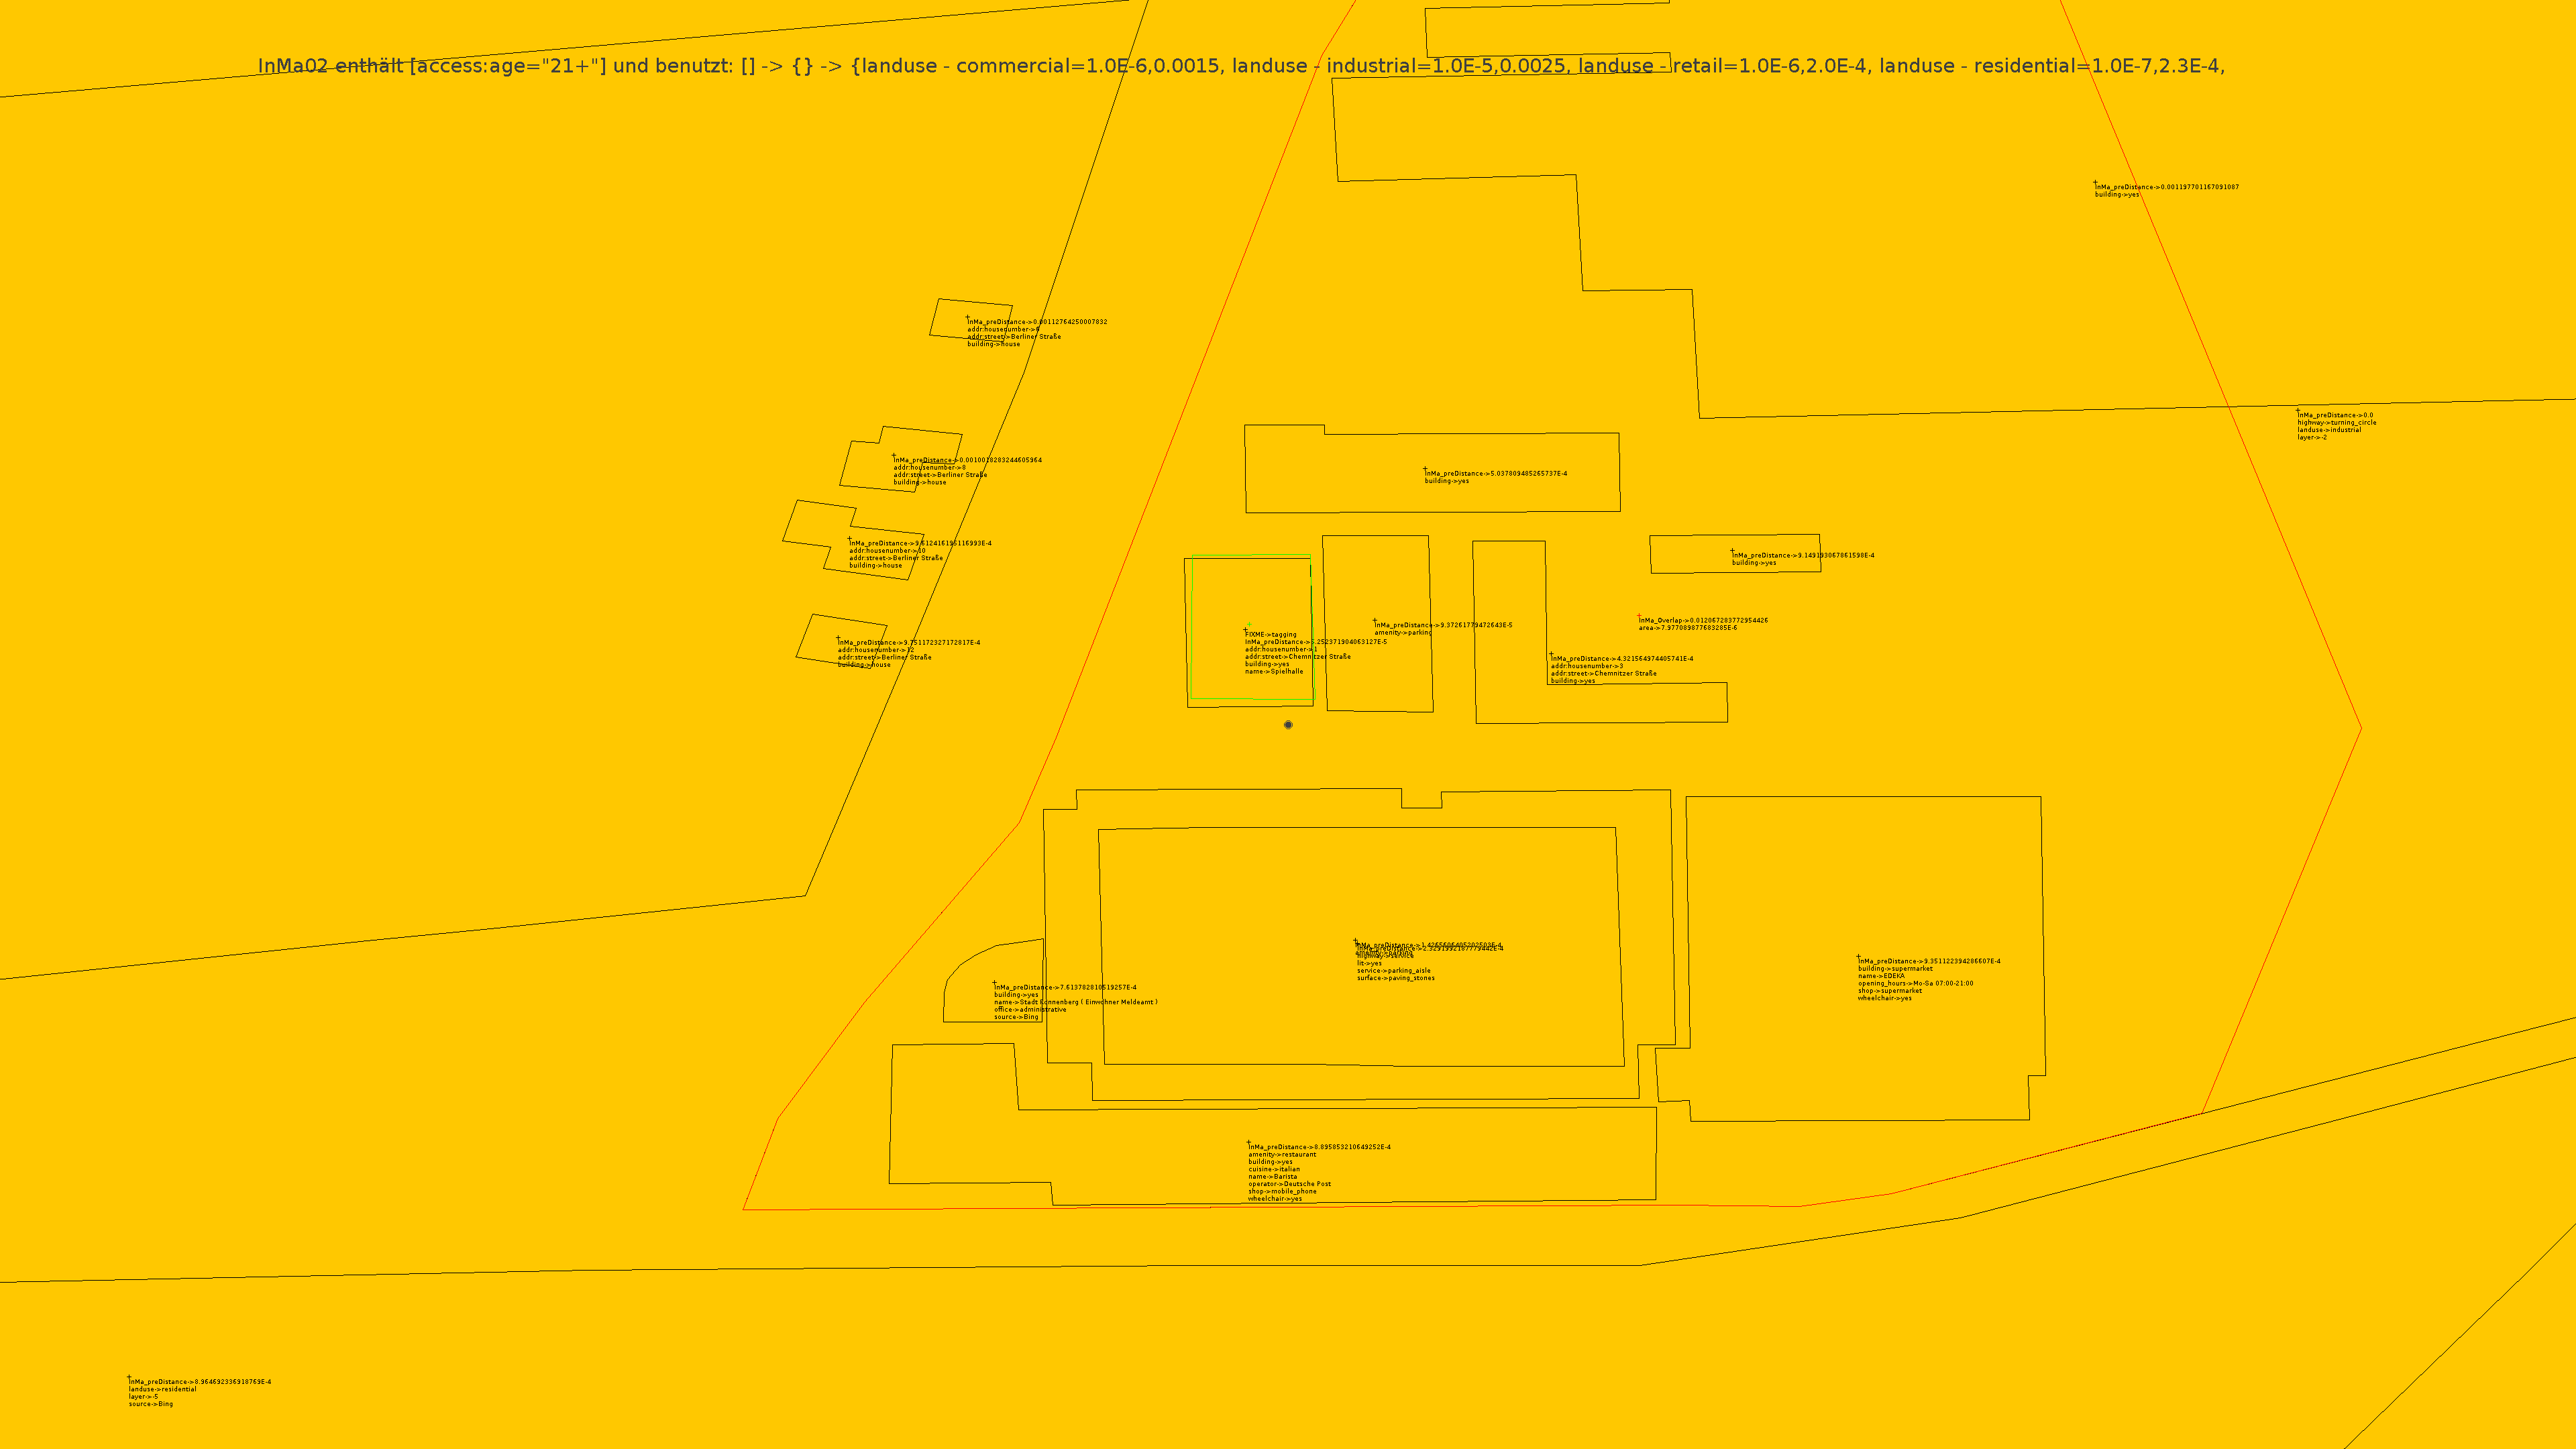
\includegraphics[width=\textwidth]{InMa02.png}
  \caption{Unvollständige Rules Definition.}
  \label{fig:NoRule}
\end{figure}

\begin{figure}
  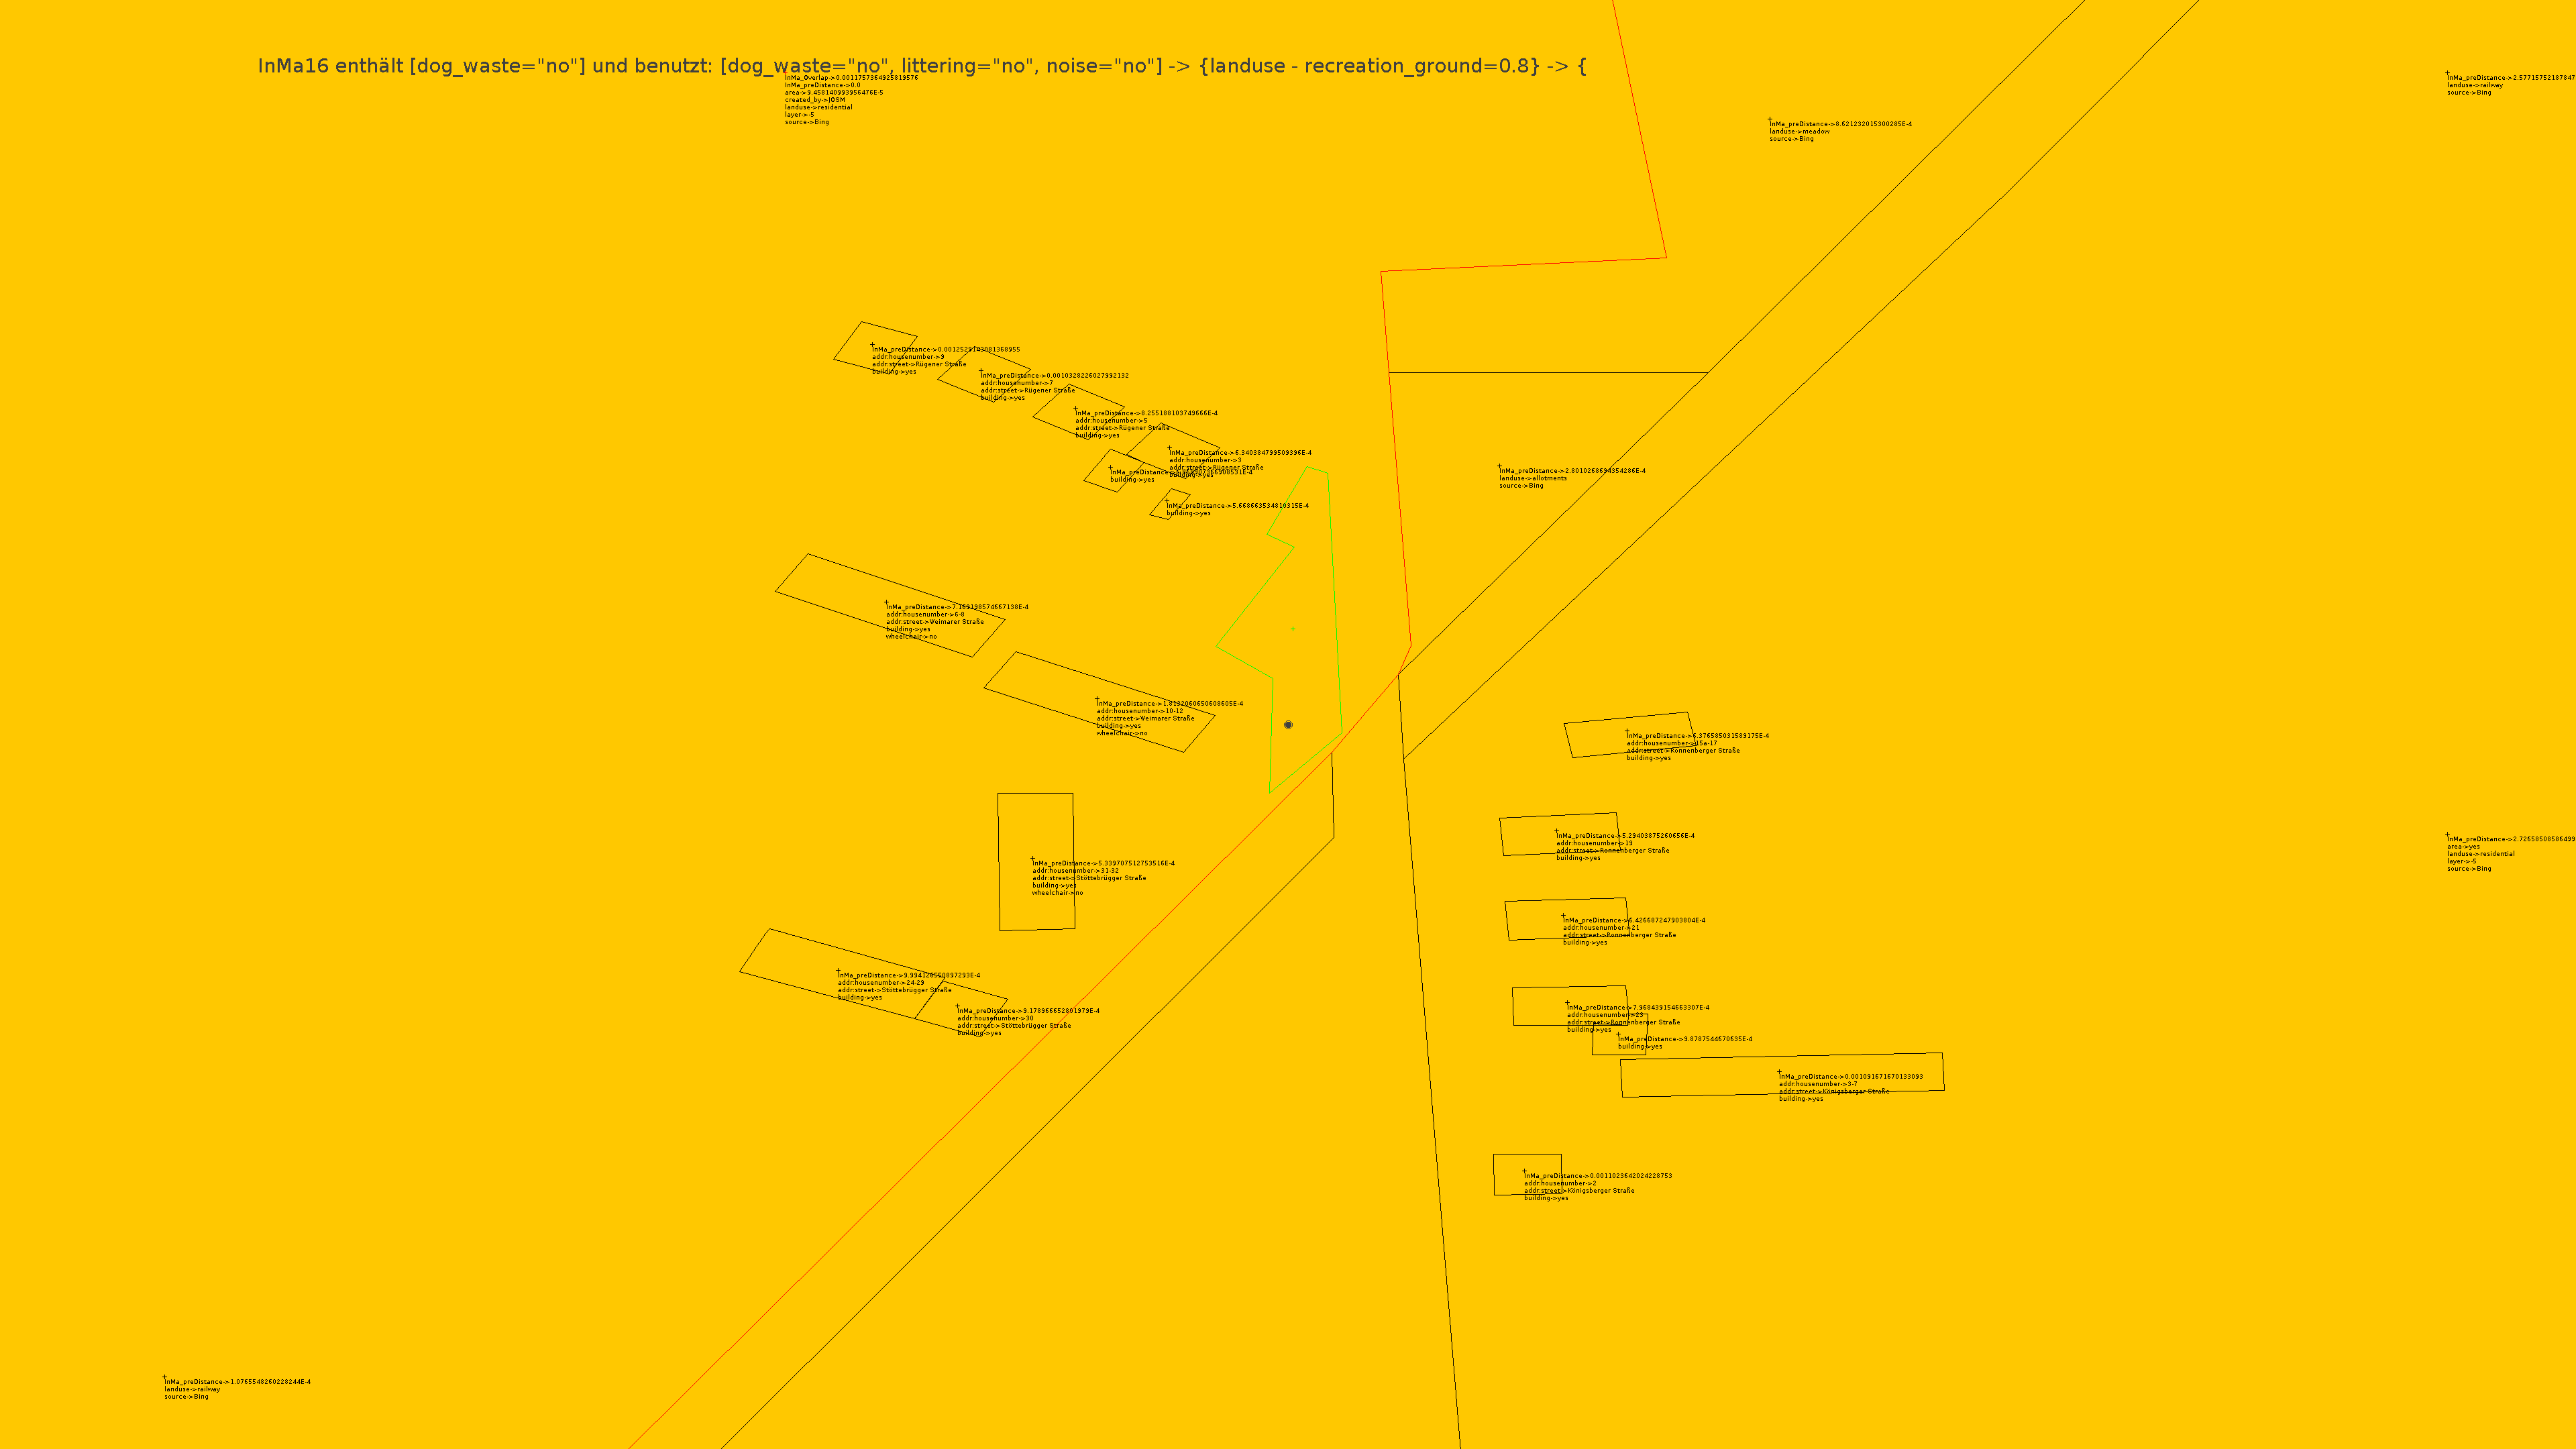
\includegraphics[width=\textwidth]{InMa16.png}
  \caption{Unvollständige Rules Einschränkungen.}
  \label{fig:MissingCircle}
\end{figure}
Das von uns bis jetzt definierte Regelwerk liefert nach einem ersten Durchlauf
zufriedenstellende Ergebnisse. Die Überlappungen sind meistens gegeben, jediglich
in 2 Fällen lag er komplett daneben. Dieses ist auf ein unvollständiges Regelwerk
aufgrund zu wenig Datansätzen zurück zu führen.

So gab es bis jetzt keine Definition für die Regel ''Zugang erst ab 21 Jahren''.
Dieses führte dazu, dass die Backup-Regel genommen wurde, das nächstebeste Polygon zu nehmen.
Da jedoch wie in \fref{fig:NoRule} zu sehen ist, das Bild vor dem gültigen Gebäude aufgenommen
wurde ist dem bisherigem Regelsatz nur noch die Regel:
\begin{lstlisting}[language=xml,frame=single]
<rule>
  <restriction>access:age="21+"</restriction>
  <OSMTag weight="0.7" >building</OSMTag>
</rule>
\end{lstlisting}
hinzuzufügen um auch diesen Datensatz vollständig zu bearbeiten.


Im zweiten Fall ist wie in \fref{fig:MissingCircle} zu sehen keine Representation
beabsichtigten Geltungsbereiches in OpenStreetMap vorhanden. Und auch wenn man davon
ausgehen kann, dass niemand gerne Hundkot vor der Nase hätte ist der beabsichtigte
Geltungsbereich für das Hinweisschild nur die Grünfläche, welche an den Parkplatz
und Strasse angrenzt.
Das Regelwerk ist also dahingehend zu ändern, dass folgende Regel hinzugefügt wird:
\begin{lstlisting}[language=xml,frame=single]
<rule>
  <restriction>dog_waste="no"</restriction>
  <OSMTag threshold="1e-8" radius="0.00023">landuse - residential</OSMTag>
</rule>
\end{lstlisting}
oder aber die bestehende Regel
\begin{lstlisting}[language=xml,frame=single]
<rule>
  <restriction>dog_waste="no"</restriction>
  <restriction>littering="no"</restriction>
  <restriction>noise="no"</restriction>
  <OSMTag weight="0.8" >landuse - recreation_ground</OSMTag>
</rule>
\end{lstlisting}
um den OSMTag erweitert wird.
Beides führt in diesem Fall zum gleichen Ergebnis.

\section{Gesamtergebnis}
\subsection{Testdatensatz}
Unser Programm und unsere Regeln führen in 61 von 96 Fällen des Testdatensatzen zu der
korrekten Lösung. In den verbleibenden 35 Datensätzen finden wir folgende Hinderlichkeiten:
\begin{itemize}
\item 9x ist das Unigebäude vorhanden, welches in OpenStreetMap nicht als einzelnes Gebäude gewertet wird.
Einen Zusammenschluss von Flächen, welche die Eigentschaft Gebäude haben und aneinander angrenzen
wäre möglich gewesen, hätte aber dazu geführt, dass viele andere Lösungen fehlerhaft werden.
\item Nr. 24, 33 Hier ist es schwierig einen Teil des Gebäudes auszugrenzen, da dieses über keine besonderen Merkmale verfügt.
\item Nr. 31 Hier ist es unmöglich für ein Programm zwischen der richtigen Lösung und falschen Lösung zu unterscheiden,
da ist es keine Metadaten in OpenStreetMap gibt, welche die beiden Flächen unterscheiden.
\item Nr. 34 Auch wenn der gegebene Lösungsbereich nicht genau getroffen wurde, so sind wir
doch mit der von uns berechneten Lösung zufrieden. Hier ist zu erkennen, dass das hinzufügen von Umkreisbeschränkungen
eine Sinnvolle Ergänzung darstellt. Der beabsichtigste Lösungsbereich wird Qualitativ getroffen.
\item Nr. 36 Hier wurde vor dem Ergänzen des Regelmenge ein ähnliches Ergebnis wie in Nr. 34 erziehlt.
Jetzt jedoch wird ein etwas falsches Gebäude ausgewählt. Wir können jedoch sagen, dass sollten
die Daten von OpenStreetMap durch weitere Gebäude erfänzt werden, so sind wir zuversichtlich, dass eine
optimale Lösungs gefunden wird.
\item Nr. 38, 39, 41, 48, 57, 60 und 61  Siehe Nr. 34. Wir sind zufrieden mit dem Ergebnis und zuversichtlich, dass
sollten mehr Daten vorhanden sein, ein optimaleres Ergebnis gefunden wird.
\item Nr. 43. Hier können wir uns den sehr kleinen Lösungsbereich Aufgrund der
gegebenen Polygone in OpenStreetMap nicht erklären. Wir empfinden unsere Lösung aber als richtig.
\item Nr. 44 Ein äusserst schwieriger Datensatz. Hier sind keine Gebäude in OpenStreetMap vorhanden
und selbst wenn, können wir aufgrund der GPS Position nicht ausschließen, dass ein
Falsches Lösungspolygon gewählt wird.
\item Nr. 45 Hier ist der mit der Fläche geschnittene Bereich etwas klein gewählt.
Dieses lässt noch Verbesserungen offen, jedoch ist hier abzuwägen wie groß das durchschnittliche
Geschäft ist, welches die Benutzung mit Fahrrädern verbietet. Diese Größe sollte berücksichtigt
werden bei Bestimmung der Schnittfläche. Wäre die GPS Koordinate in der Mitte des Gebäudes
platziert, so hätte sich eine fast optimale Lösung ergeben.
\item Nr. 49 Hier hat unser Algorithmus komplett versagt. Auch nach etlichen Überlegungen
sind wir zu keinem Ergebnis gekommen, das uns zufriedenstellen würde.
\item Nr. 50 Hier hat der Algorithmus etwas daneben gegriffen, aber man kann erkennen,
dass unsere Lösung nicht allzu weit entfernt ist von der Musterlösung. Eine zusammenfassung von Gebäuden
hätte auch hier helfen können, hätte jedoch auch nicht das optimale Lösungspolygon ergeben.

\item Nr. 51 Eine weiteres sehr schwierige Problem. Hier hätte eine bessere Lösung gefunden werden können,
Wenn man den Gebäudekomplex mit einer quadratischen Fläche ähnlich den angrenzenden Gebäuden schneidet.
Dieses ist jedoch eine höchst komplexe Aufgabe und würde auch nicht den Erfolg garantieren.
Besser wäre es, wenn OpenStreetMap mehr Daten hätte.

\item Nr. 53. Aufgrund der Tatsache, dass hier keine Daten in OpenStreetMap vorhanden sind
sind wir sehr zufrieden mit dem Ergebnis. Es wurde keines der Angrenzenden Gebäude ausgewählt,
sondern ein Bereich von ungefähr der Gesuchten Größe mit nur etwas verschobener Position.

\item Nr. 55 Der Gewählte Bereich ist etwas zu groß gewählt, hier ist der Gegenpol zu Nr. 45.
\item Nr. 56 Aufgrund der Fehlenden Daten in OpenStreetMap die nächstbeste und aufgrund der Daten
auch sinnvolle Lösung. Wenn man nicht wüsste, dass es falsch ist, so würde ein Mensch dieses wahrscheinlich
auch auswählen.

\item Nr. 58 und 59 Hier ist zu sagen: Pech gehabt. Wäre die Koordinate etwas näher an der andere Fläche
oder das Gebäude in OpenStreetMap vorhanden, wäre die Lösung besser gewesen.
\item Nr. 62 Hier können wir Musterlösung und Datenlage nicht vernünftig interpretieren und bewerten.
\item Nr. 79 Hier scheinen die Daten von OpenStreetMap und der Musterlösung zu divergieren. Unter den
gegebenen Umständen ist die von uns gewählte Lösung als Richtig anzusehen.
\end{itemize}
\subsection{Eigene Daten}
Auch hier sind wir zufrieden mit den Ergebnissen. Auch wenn nicht immer die Optimalen Ergebnisse
gefunden wurden, so sind diese doch brauchbar und es mussten nur einige wenige Anpassungen
an den Regeln vorgenommen werden.
Bedingt durch die vielen kleinen Geschäfte, welche sich in Teilbereichen von Häusern befinden ist es schwierig
deren genauen Umriss zu erstellen.
Es hat sich hier für uns gezeigt, dass einiges an Arbeit in OpenStreetMap gesteckt werden kann und
uns ermuntert dieses auch zu tun.


Zusammenfassend ist zu sagen, dass wir bis auf einige wenige Ausrutscher mit der
Qualität der Lösungen zufrieden sind.
